\documentclass[12pt,a4paper]{report}

% Typography and page layout follow the project report template.
\usepackage[utf8]{inputenc}
\usepackage[T1]{fontenc}
\usepackage{amsmath,amssymb}
\usepackage[lining]{ebgaramond}
\usepackage[cmintegrals,cmbraces]{newtxmath}
\usepackage{microtype}
\usepackage{geometry}
\usepackage{graphicx}
\usepackage{booktabs}
\usepackage{tabularx}
\usepackage{array}
\usepackage{caption}
\usepackage{float}
\usepackage{enumitem}
\usepackage{xcolor}
\usepackage{hyperref}
\usepackage{titlesec}
\usepackage{url}

\graphicspath{{../figure/}}
\AtBeginDocument{\fontsize{13}{15.6}\selectfont}
\geometry{left=1.8cm,right=1.8cm,top=2.2cm,bottom=2.2cm}
\definecolor{crimson}{RGB}{153,0,0}
\hypersetup{colorlinks=true,linkcolor=crimson,citecolor=crimson,urlcolor=crimson}
\tolerance=2000
\emergencystretch=2em
\setlength{\parindent}{0pt}
\setlength{\parskip}{0.35em}
\setlength{\floatsep}{6pt plus 2pt minus 2pt}
\setlength{\textfloatsep}{10pt plus 2pt minus 2pt}
\setlength{\intextsep}{10pt plus 2pt minus 2pt}
\captionsetup[figure]{skip=5pt,belowskip=2pt}
\captionsetup[table]{skip=3pt}
\titleformat{\chapter}{\normalfont\huge\bfseries}{}{0pt}{}[\vspace{0.3em}]
\titlespacing*{\chapter}{0pt}{0pt}{14pt}
\titleformat{\section}{\normalfont\Large\bfseries}{\thesection}{1em}{}
\titleformat{\subsection}{\normalfont\large\bfseries}{\thesubsection}{1em}{}

\newcommand{\msr}{\mathrm{MSR}}
\newcommand{\msrfour}{\mathrm{MSR\text{-}4}}
\newcommand{\concat}{\mathbin\Vert}
\newcommand{\bvec}[1]{\mathbf{#1}}
\edef\msrcalfigure{\detokenize{MSR&CAL.png}}

\begin{document}
\pagestyle{plain}

\begin{titlepage}
\centering
\vspace*{3cm}
{\fontsize{28}{34}\selectfont\bfseries Low-Cost AI Accelerator\par}
\vspace{0.6em}
{\fontsize{20}{26}\selectfont\bfseries Design Specification\par}
\vspace{0.4em}
{\fontsize{16}{22}\selectfont\bfseries MSR-4 Weight Encoding and Compensation\par}

\vspace{1.5cm}
\textcolor{crimson}{\rule{0.6\linewidth}{1.2pt}}\par
\vspace{1.5cm}

{\large\bfseries Current scope}\par
\vspace{0.4em}
{\large Introduction, Background, and Motivation}\par

\vfill
\textcolor{crimson}{\rule{0.6\linewidth}{0.6pt}}\par
\vspace{0.5em}
{\small The architecture, control, verification, and PPA chapters will be added as the project progresses.}\par
\end{titlepage}

\tableofcontents
\newpage

\chapter{Introduction}
\label{ch:introduction}

\textit{This section is reserved for the project problem statement, contributions, and document organization. It will be completed after the proposed architecture and evaluation scope are finalized.}

\chapter{Background}
\label{ch:background}

\section{INT8 Quantization for DNN Inference}

Deep neural networks are normally trained with floating-point arithmetic, but the cost of floating-point weights and MAC operations is often unnecessary during inference. A signed INT8 representation reduces weight storage, memory traffic, and multiplier complexity while retaining a practical accuracy baseline. Let $w$ be a floating-point weight and $s$ be the quantization scale. The signed integer weight used by the accelerator is
\begin{equation}
    q=\operatorname{clip}_{[-128,127]}\bigl(\operatorname{round}(s w)\bigr),
    \label{eq:int8-quantization}
\end{equation}
where $q$ is stored as an 8-bit two's-complement word. For an activation vector $\bvec{x}$ and a quantized weight vector $\bvec{q}$, the INT8 reference operation is
\begin{equation}
    y=\sum_{i=0}^{K-1}x_iq_i.
    \label{eq:int8-dot-product}
\end{equation}

INT8 treats every weight with the same storage width and multiplier interface, even though the bit patterns of trained weights are not uniformly distributed. In particular, weights close to zero contain redundant sign-extension bits after quantization. The proposed design exploits this representation-level redundancy while retaining INT8 as the external quantization interface and the accuracy reference.

\section{Most Significant Runs}

For an $N$-bit two's-complement word, an MSR-$k$ pattern is a run of $k$ identical bits at the most significant end. This specification uses $N=8$ and selects $k=4$. Let
\begin{equation}
    q=(b_7b_6b_5b_4b_3b_2b_1b_0)_2,
\end{equation}
where $b_7$ is the sign bit. The MSR-4 predicate is
\begin{equation}
    \mathcal{M}_4(q)=1 \Longleftrightarrow b_7=b_6=b_5=b_4.
    \label{eq:msr4-predicate}
\end{equation}
Thus, both $0000xxxx_2$ and $1111xxxx_2$ are MSR-4 values. Figure~\ref{fig:msr-quantization} illustrates why the pattern is common after fixed-point quantization: small positive values generate leading zeros, while small negative values generate leading ones.

\begin{figure}[H]
    \centering
    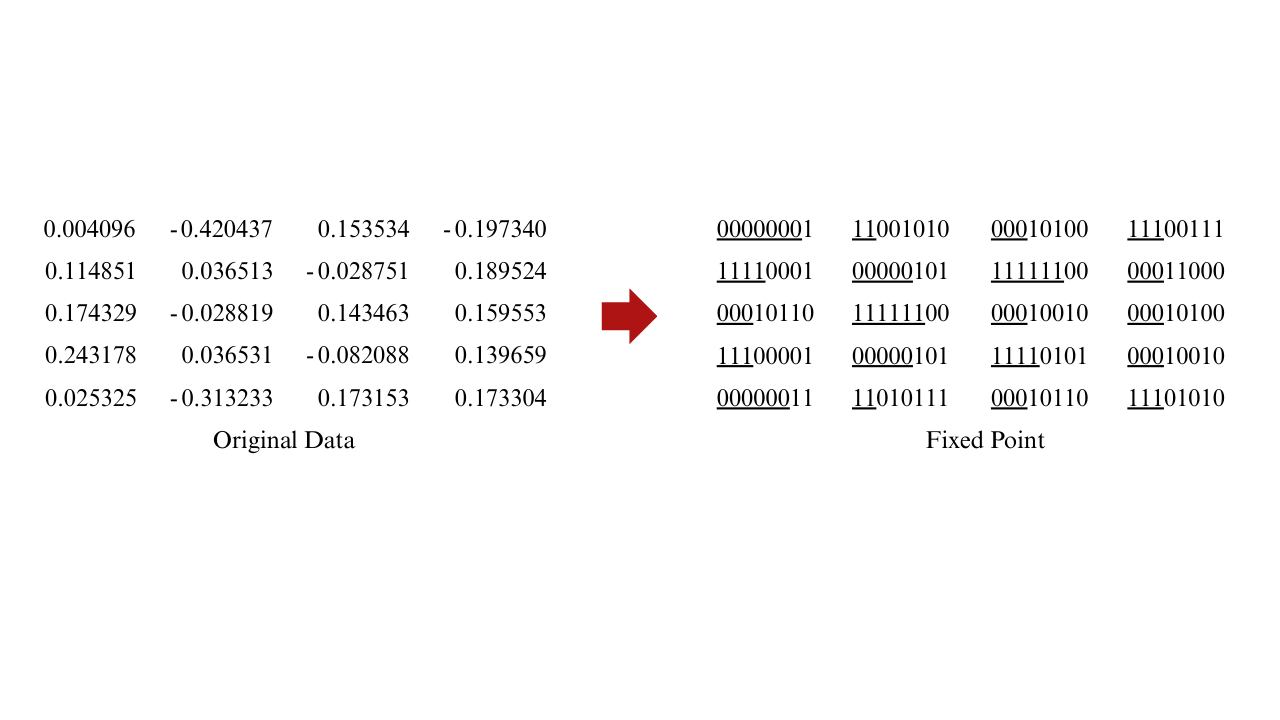
\includegraphics[width=0.96\textwidth]{MSR.png}
    \caption{Example conversion from floating-point weight data to fixed-point words. Underlined leading bits illustrate MSR candidates.}
    \label{fig:msr-quantization}
\end{figure}

For example, with scale $s=128$, $0.10534$ maps to $13=(00001101)_2$ and has four leading zeros. Similarly, $-0.0784$ maps to $-10=(11110110)_2$ and has four leading ones. In both cases, the four most significant bits independently carry no additional information once the remaining field and the class are known.

\section{MSR-4 Weight Encoding}

The Weight Pre-processing Unit (WPU) classifies every INT8 weight using \eqref{eq:msr4-predicate}. It emits one 5-bit reduced word $r$ for the main array and a compensation-valid bit $v_c$. The corresponding encoding is defined in Table~\ref{tab:weight-encoding}. The leading bit of $r$ is a class tag: zero identifies an MSR-4 reduced word and one identifies a non-MSR-4 high-nibble contribution.

\begin{table}[H]
\centering
\caption{MSR-4-Aware Per-Weight Encoding}
\label{tab:weight-encoding}
\renewcommand{\arraystretch}{1.2}
\setlength{\tabcolsep}{10pt}
\begin{tabularx}{\textwidth}{>{\centering\arraybackslash}p{2.1cm}>{\centering\arraybackslash}X>{\centering\arraybackslash}X>{\centering\arraybackslash}p{1.0cm}}
\toprule
\textbf{Class} & \textbf{Reduced word $r$} & \textbf{Compensation word $c$} & \textbf{$v_c$} \\
\midrule
MSR-4 & $0\concat b_4b_3b_2b_1$ & Not consumed by the CPE & 0 \\
Non-MSR-4 & $1\concat b_7b_6b_5b_4$ & $b_7\concat b_3b_2b_1$ & 1 \\
\bottomrule
\end{tabularx}
\end{table}

For an MSR-4 weight, bits $b_4$ through $b_1$ are retained and $b_0$ is reconstructed as one in the local MAC datapath. The reduced-path value is therefore
\begin{equation}
    \hat{q}_{\msrfour}=2\,\operatorname{sext}_4(b_4b_3b_2b_1)+1.
    \label{eq:msr4-reconstruction}
\end{equation}
This expected-value LSB rule enables the five-bit representation without carrying the original LSB through every Reduced Processing Element (RPE). A non-MSR-4 weight retains its high-nibble contribution in the RPE path and carries its omitted signed residual in the Compensation Processing Element (CPE) path. The two partial products are accumulated only when $v_c=1$.

\chapter{Motivation}
\label{ch:motivation}

\section{Why MSR-4 Is the Selected Operating Point}

The MSR length determines the trade-off between compression opportunity and the frequency of compensation. Table~\ref{tab:msr-coverage} summarizes the measured MSR coverage of four INT8-quantized MNIST models. MSR-3 is nearly universal but preserves fewer redundant bits. MSR-5 through MSR-7 provide more aggressive reduction, but their coverage becomes model dependent; LeNet falls to $88.3\%$ at MSR-5 and $53.4\%$ at MSR-6. MSR-4 provides the selected balance: it covers at least $98.90\%$ of the reported weights while supporting the 5-bit reduced representation in Table~\ref{tab:weight-encoding}.

\begin{table}[H]
\centering
\caption{Observed MSR Coverage of INT8 Weight Data}
\label{tab:msr-coverage}
\renewcommand{\arraystretch}{1.18}
\setlength{\tabcolsep}{12pt}
\begin{tabular}{lrrrr}
\toprule
\textbf{Run criterion} & \textbf{MLP} & \textbf{LeNet} & \textbf{ResNet} & \textbf{AlexNet} \\
\midrule
MSR-3 & 99.9\% & 99.9\% & 99.9\% & 99.9\% \\
MSR-4 & 99.98\% & 98.90\% & 99.61\% & 99.98\% \\
MSR-5 & 98.0\% & 88.3\% & 99.5\% & 99.7\% \\
MSR-6 & 78.2\% & 53.4\% & 99.1\% & 97.8\% \\
MSR-7 & 40.4\% & 27.3\% & 85.5\% & 84.3\% \\
\bottomrule
\end{tabular}
\end{table}

\section{MSR-4 Exception Density and Compensation Capacity}

The low non-MSR-4 density makes a sparse compensation array practical. For a column with $N=256$ weights and MSR-4 coverage $p_{\msrfour}$, the expected number of non-MSR-4 weights is
\begin{equation}
    E[N_{\mathrm{non}}]=N(1-p_{\msrfour}).
    \label{eq:exception-density}
\end{equation}
LeNet is the limiting model in the reported data. With $p_{\msrfour}=0.9890$,
\begin{equation}
    E[N_{\mathrm{non}}]=256(1-0.9890)=2.816\approx2.9.
    \label{eq:lenet-exceptions}
\end{equation}
Accordingly, the target $256\times256$ reduced-precision systolic array is paired with a $256\times3$ compensation array. The latter contains 768 CPE sites, only $768/65{,}536\approx1.17\%$ of the main-array site count. This ratio does not directly represent area or power overhead, but it establishes that the correction resource can remain narrow when the measured MSR-4 distribution is maintained.

The average in \eqref{eq:lenet-exceptions} is not a worst-case bound. The model-preparation flow shall count non-MSR-4 weights for every mapped tile and column before preload. A column with more than three exceptions must be reported as an overflow and scheduled by a separate mapping or compensation pass; it must not silently discard the excess residuals.

\section{Expected-Value Approximation and Sparse Compensation}

Setting the discarded LSB to one intentionally introduces a bounded approximation for an MSR-4 weight:
\begin{equation}
    \epsilon_q=\hat{q}-q=1-b_0.
    \label{eq:lsb-error}
\end{equation}
For a dot product consisting of MSR-4 values, this error accumulates as
\begin{equation}
    \epsilon_y=\sum_i x_i(1-b_{0,i}).
    \label{eq:dot-product-error}
\end{equation}
The assumption must consequently be evaluated with an RTL-equivalent model and compared with INT8 inference; MSR coverage alone is not an accuracy result.

Non-MSR-4 values require a separate mechanism because reducing them only to their high nibble discards information that can materially affect sensitive layers. The CPE path retains the sign and lower residual field for these exceptional weights, while the main RPE array processes the common case. Figure~\ref{fig:msr-calculation} summarizes the data decomposition, storage, reduced-precision MAC operation, and correction accumulation that motivate this split.

\begin{figure}[H]
    \centering
    \includegraphics[width=0.96\textwidth]{\msrcalfigure}
    \caption{MSR-4-aware weight processing and sparse compensation. MSR-4 weights use the reduced path; non-MSR-4 weights produce a reduced contribution and a compensation contribution that are merged in the accumulator.}
    \label{fig:msr-calculation}
\end{figure}

\section{Verification Implications}

The WPU behavior follows directly from Table~\ref{tab:weight-encoding}. The following representative vectors shall be observed: $00001101_2$ produces $r=00110_2$ and $v_c=0$; $11110110_2$ produces $r=01011_2$ and $v_c=0$; and $01010110_2$ produces $r=10101_2$, $c=0011_2$, and $v_c=1$. The WPU verification plan shall exhaustively cover all 256 INT8 input words in addition to these representative vectors.

\begin{thebibliography}{9}
\bibitem{project-readme}
``Low-Cost AI Accelerator Based on TPU v1,'' project README, \texttt{tpu-accelerator-lite}, accessed July 2026.

\bibitem{weight-aware-thesis}
``Weight-Aware and Reduced-Precision Architecture Designs for Low-Cost AI Accelerators,'' National Taiwan University of Science and Technology repository. [Online]. Available: \url{https://hdl.handle.net/11296/zs6qk8}
\end{thebibliography}

\end{document}
